% gc-02-Limits.tex

\documentclass[xcolor=dvipsnames]{beamer}

\usepackage{cancel}
\renewcommand{\CancelColor}{\color{red}}
\usepackage{graphicx}
\usepackage{wrapfig}
\usepackage{colortbl}
\definecolor{myblue}{rgb}{0.8,0.85,1}

\mode<presentation>
{
  \usetheme{Warsaw}
  \setbeamercovered{transparent}
}
% \usecolortheme[named=OliveGreen]{structure}
\setbeamertemplate{navigation symbols}{} 
\setbeamertemplate{blocks}[rounded][shadow=true] 

\newif\ifBCITCourse
\BCITCoursetrue
% \BCITCoursefalse
\newif\ifWhichCourse
\WhichCoursetrue
\WhichCoursefalse
\ifBCITCourse
\ifWhichCourse
\newcommand{\CourseName}{Statistics for Food Technology}
\newcommand{\CourseNumber}{MATH 2441}
\newcommand{\CourseInst}{BCIT}
\else
\newcommand{\CourseName}{Calculus for Geomatics}
\newcommand{\CourseNumber}{MATH 2511}
\newcommand{\CourseInst}{BCIT}
\fi
\else
\newcommand{\CourseName}{Philosophy and Literature}
\newcommand{\CourseNumber}{PHIL 375}
\newcommand{\CourseInst}{UBC}
\fi

\title{Limits}
\subtitle{{\CourseNumber}, BCIT}

\author{\CourseName}

\date{January 8, 2018}

% \begin{figure}[h]
% 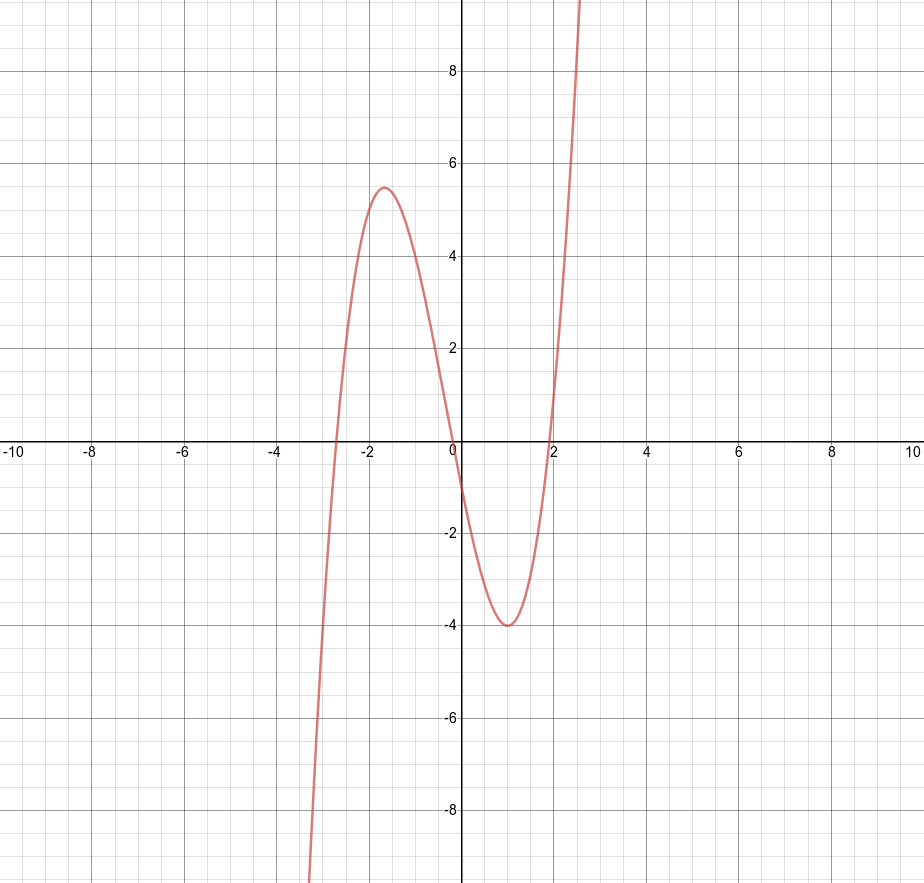
\includegraphics[scale=.3]{./extrema1.png}
% \end{figure}

\begin{document}

\begin{frame}
  \titlepage
\end{frame}

\begin{frame}
  \frametitle{Limits Introduction}
Consider the function graph of the following function.
\begin{equation}
  \label{eq:quiekong}
  f(x)=\frac{x^{2}-1}{x-1}
\end{equation}
It looks like it is a linear equation! However, at $x=1$, $f(x)$ is
not defined. To fill the hole, we define the limit
\begin{equation}
  \label{eq:vaineiro}
  \lim_{x\rightarrow{}a}f(x)=w\mbox{ if and only if }w=L=R
\end{equation}
where $L$ is the number that the function $f$ approaches as $x$ gets
closer to $a$ with $x<a$ (that means $x\neq{}a$!); and $R$ is the
number that the function $f$ approaches as $x$ gets closer to $a$ with
$x>a$. Note: for a mathematically rigorous definition of what
``approaching'' and ``getting closer'' means we would need to
talk about sequences and series, which is a topic we won't cover here.
\end{frame}

\begin{frame}
  \frametitle{Indeterminate Form I}
Notice that
\begin{equation}
  \label{eq:iicheeci}
  f(x)=\frac{x^{2}-1}{x-1}\overset{x=1}{=}\frac{0}{0}
\end{equation}
We call this an \alert{indeterminate form}.
\end{frame}

\begin{frame}
  \frametitle{Indeterminate Form}
Notice that except at $x=1$
\begin{equation}
  \label{eq:dooshool}
  f(x)=\frac{x^{2}-1}{x-1}=\frac{\cancel{(x-1)}(x+1)}{\cancel{x-1}}=x+1=g(x)
\end{equation}
$f$ and $g$ agree everywhere except on $x=1$. Consider the following
rule,
\begin{block}{One Disagreement Rule}
If $f=g$ except in one point, then
$\lim_{x\rightarrow{}a}f(x)=\lim_{x\rightarrow{}a}g(x)$ for all $a$,
even the $a$ where $f$ and $g$ disagree.
\end{block}
Therefore
\begin{equation}
  \label{eq:eengemia}
  \lim_{x\rightarrow{}1}\frac{x^{2}-1}{x-1}=\lim_{x\rightarrow{}1}(x+1)=2
\end{equation}
\end{frame}

\begin{frame}
  \frametitle{Continuity}
Consider a simple function like $f(x)=x^{3}$. What is
$\lim_{x\rightarrow{}4}f(x)$? The answer is almost trivial,
\begin{equation}
  \label{eq:zaethahv}
  \lim_{x\rightarrow{}4}f(x)=f(4)=4^{3}=64
\end{equation}
Why is this true? Because $f$ is continuous at $x=4$. There are no
holes, jumps, gaps, or breaks of the function graph at $x=4$. 
% In fact,
% $f$ is continuous on the whole domain of $f$. A function is
% \alert{continuous} at $x=a$ if and only if (1) $f(a)$ is defined; (2)
% $\lim_{x\rightarrow{}a}f(x)$ exists; and (3)
% $\lim_{x\rightarrow{}a}f(x)=f(a)$. 
Constant functions, the identity function, linear functions,
polynomial functions, exponential and logarithmic functions are all
continuous. Rational functions, some trigonometric functions, and
other functions are sometimes \alert{not} continuous.
\end{frame}

\begin{frame}
  \frametitle{Interesting Cases}
  A function is continuous if and only if
  $\lim_{x\rightarrow{}c}f(x)=f(c)$ for all $c$ in $\mathbb{R}$ (the
  logarithmic function is continuous only on $\mathbb{R}^{+}$).
  This means that (i) the function needs to be defined at $x=c$; (ii)
  the limit needs to be defined at $x=c$; and (iii) the function value
  and the limit need to be equal to each other.

Consider the following interesting cases:
\begin{enumerate}
\item<1-> A function that is continuous and well defined at $x=a$.
\item<2-> A function that is not continuous at $x=a$.
\item<3-> A function where the limit exists but $\lim_{x\rightarrow{}c}\neq{}f(c)$.
\item<4-> A function such as $f(x)=\sin(1/x)$.
\end{enumerate}
\end{frame}

% \begin{frame}
%   \frametitle{Informal Definition of Limit}
% The function $f$ has the \alert{limit} $L$ as $x$ approaches $a$,
% written
% \begin{equation}
%   \label{eq:beiquoob}
%   \lim_{x\rightarrow{}a}f(x)=L
% \end{equation}
% if the value of $f(x)$ can be made as close to the number $L$ as we
% please by taking $x$ sufficiently close to (but not equal to) $a$.
% \end{frame}

\begin{frame}
  \frametitle{No Limit Examples I}
  \begin{figure}[h]
    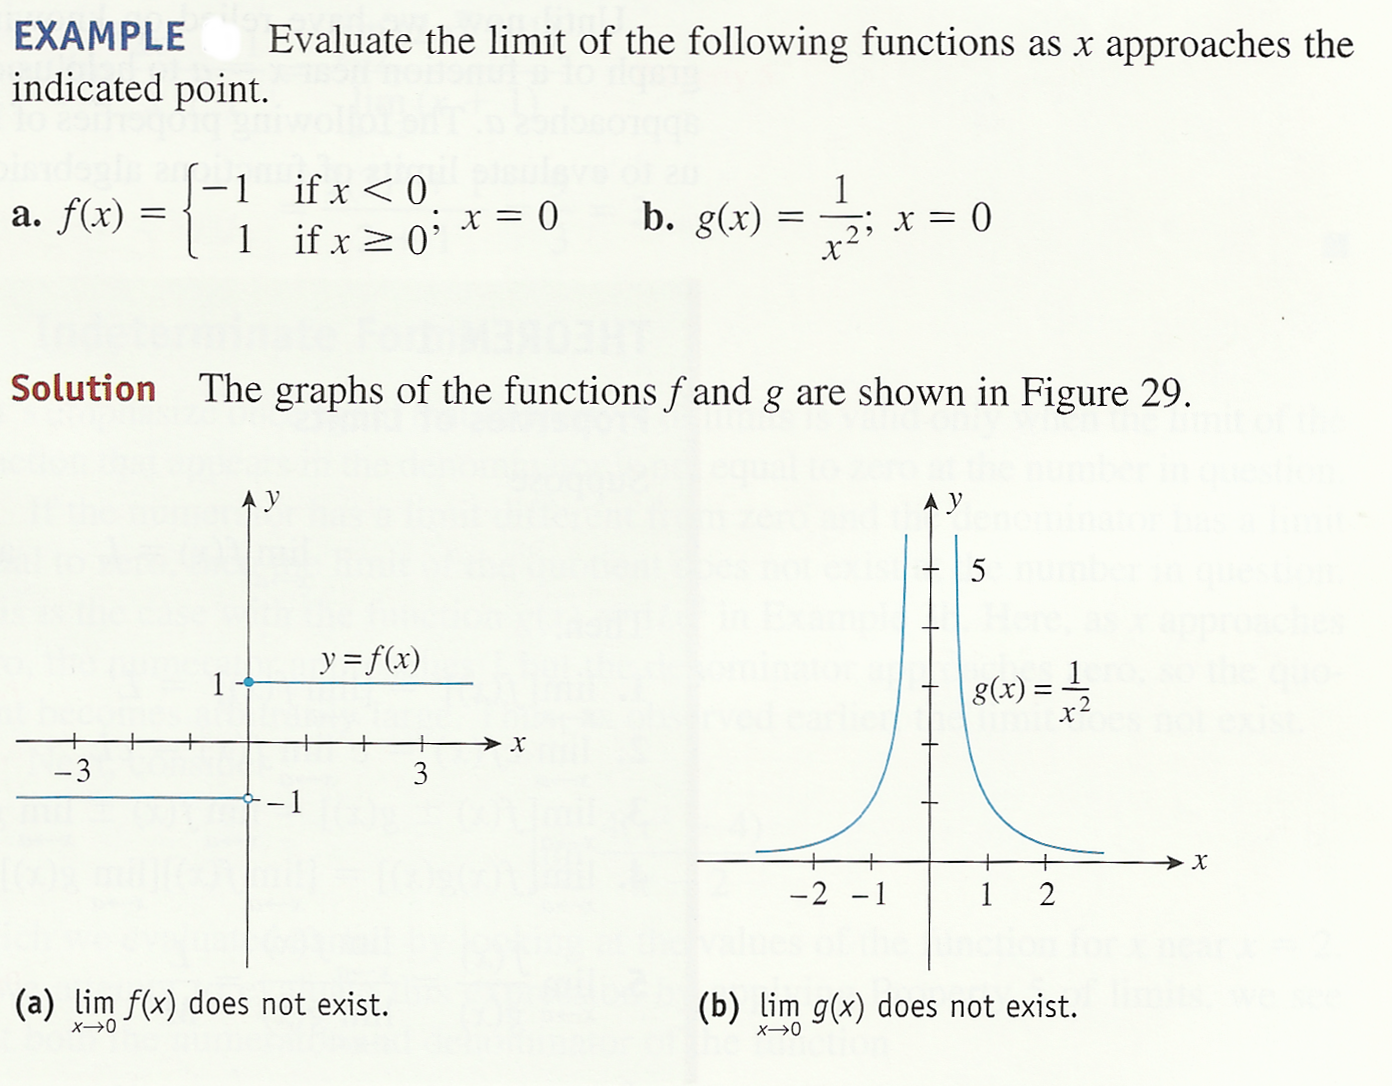
\includegraphics[scale=.9]{./limita.png}
  \end{figure}
\end{frame}

\begin{frame}
  \frametitle{No Limit Example II}
  \begin{figure}[h]
    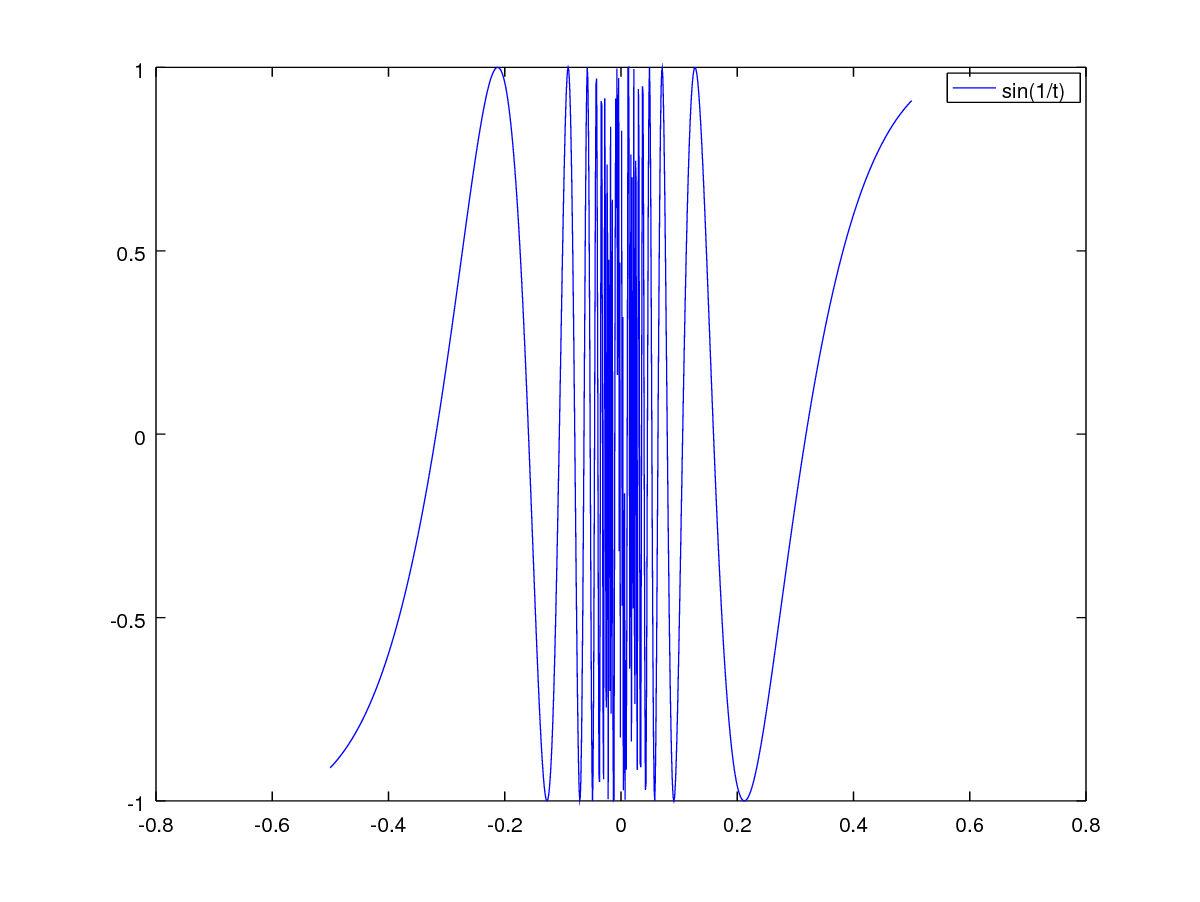
\includegraphics[scale=.5]{./sineoneoverx.png}
  \end{figure}
\end{frame}

\begin{frame}
  \frametitle{Properties of Limits}
  Suppose $\lim_{x\rightarrow{}a}f(x)=L$ and
  $\lim_{x\rightarrow{}a}g(x)=M$. Then (call this \alert{Theorem 1}),
\begin{equation}
  \label{eq:johvoohu}
  \lim_{x\rightarrow{}a}[f(x)]^{r}=L^{r},r\mbox{ a real number}
\end{equation}
\begin{equation}
  \label{eq:eeyootoh}
  \lim_{x\rightarrow{}a}[c\cdot{}f(x)]=c\cdot{}L,c\mbox{ a real number}
\end{equation}
\begin{equation}
  \label{eq:kohzahwa}
  \lim_{x\rightarrow{}a}[f(x)\pm{}g(x)]=L\pm{}M
\end{equation}
\begin{equation}
  \label{eq:aekaqued}
  \lim_{x\rightarrow{}a}[f(x)g(x)]=LM
\end{equation}
\begin{equation}
  \label{eq:ahkeigae}
  \lim_{x\rightarrow{}a}\frac{f(x)}{g(x)}=\frac{L}{M},\mbox{provided that }M\neq{}0
\end{equation}
\end{frame}

\begin{frame}
  \frametitle{Properties of Limits Exercises}
Use the properties of limits to evaluate the following,
\begin{equation}
  \label{eq:eemoopha}
 \lim_{x\rightarrow{}2}x^{3} 
\end{equation}
\begin{equation}
  \label{eq:queebaet}
 \lim_{x\rightarrow{}4}5x^{3/2} 
\end{equation}
\begin{equation}
  \label{eq:xoquaenu}
 \lim_{x\rightarrow{}1}\left(5x^{4} -2\right)
\end{equation}
\begin{equation}
  \label{eq:othahzau}
 \lim_{x\rightarrow{}3}2x^{3}\sqrt{x^{2}+7}
\end{equation}
\begin{equation}
  \label{eq:ayaivoma}
 \lim_{x\rightarrow{}2}\frac{2x^{2}+1}{x+1}
\end{equation}
\end{frame}

\begin{frame}
  \frametitle{Another Indeterminate Form Example I}
  Here is an example where by skillful manipulation we can determine
  the limit even though at first the limit is in indeterminate form.
  Let
\begin{equation}
  \label{eq:xierigai}
  f(x)=\frac{\sqrt{1+x}-1}{x}
\end{equation}
What is $\lim_{x\rightarrow{}0}f(x)$? If we leave the fraction
unchanged, it will give us an indeterminate form. However, if we
multiply both numerator and denominator by $(\sqrt{1+x}+1)$, we avoid
the indeterminate form!
\begin{equation}
  \label{eq:ciabohmi}
  \lim_{x\rightarrow{}0}f(x)=\lim_{x\rightarrow{}0}\frac{\sqrt{1+x}-1}{x}=\lim_{x\rightarrow{}0}\frac{1}{\sqrt{1+x}+1}=\frac{1}{\sqrt{1}+1}=\frac{1}{2}
\end{equation}
Look at the function graph of $f(x)$ to verify that this is the
correct limit.
\end{frame}

\begin{frame}
  \frametitle{Another Indeterminate Form Example II}
  \begin{figure}[h]
    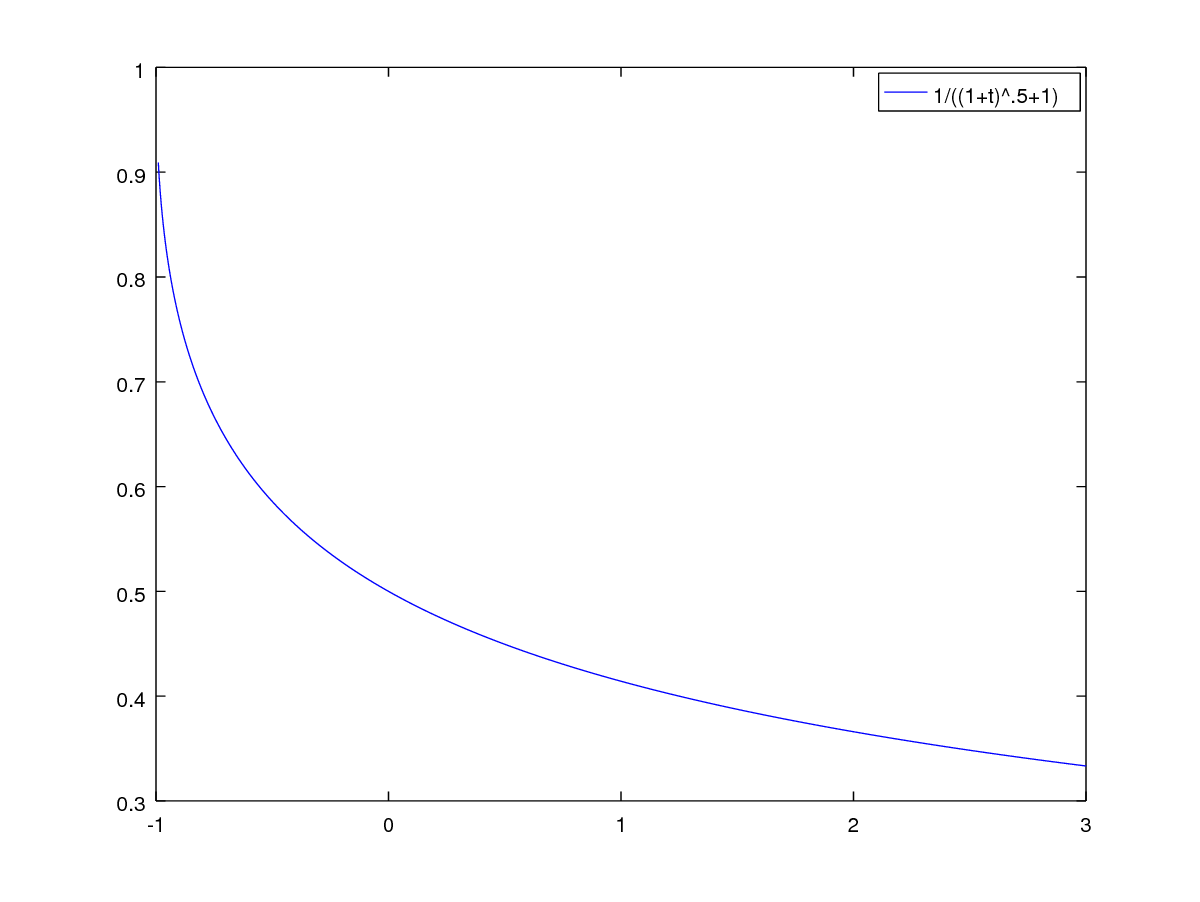
\includegraphics[scale=.5]{./indeterminate.png}
  \end{figure}
\end{frame}

\begin{frame}
  \frametitle{Limits at Infinity I}
Sometimes, we want to know what happens to a function graph when
either $x$ or $-x$ get very large. We use the infinity sign $\infty$
for notation, but note that we do NOT use infinity to define these
limits. 
\begin{equation}
  \label{eq:xetieshe}
  \lim_{x\rightarrow{}\infty}f(x)=w\mbox{ if and only if }w=S
\end{equation}
where $S$ is a number such that for any tiny number $\varepsilon$
there is a real number $x_{0}$ and
$\vert{}f(x)-S\vert<\varepsilon$ for all $x>x_{0}$.
\end{frame}

\begin{frame}
  \frametitle{Limits at Infinity II}
% Sometimes, we want a limit not at $x=a$ but as $x$ goes to positive or
% negative infinity (i.e.\ increases or decreases without bound). We use
% the symbol $\infty$ for infinity. 
For example, what is
\begin{equation}
  \label{eq:wingeisa}
  \lim_{x\rightarrow\infty}\frac{2x^{2}}{1+x^{2}}
\end{equation}
or
\begin{equation}
  \label{eq:ahxaibah}
  \lim_{x\rightarrow{}-\infty}\frac{2x^{2}}{1+x^{2}}
\end{equation}
\end{frame}

\begin{frame}
  \frametitle{Limits at Infinity III}
  \begin{figure}[h]
    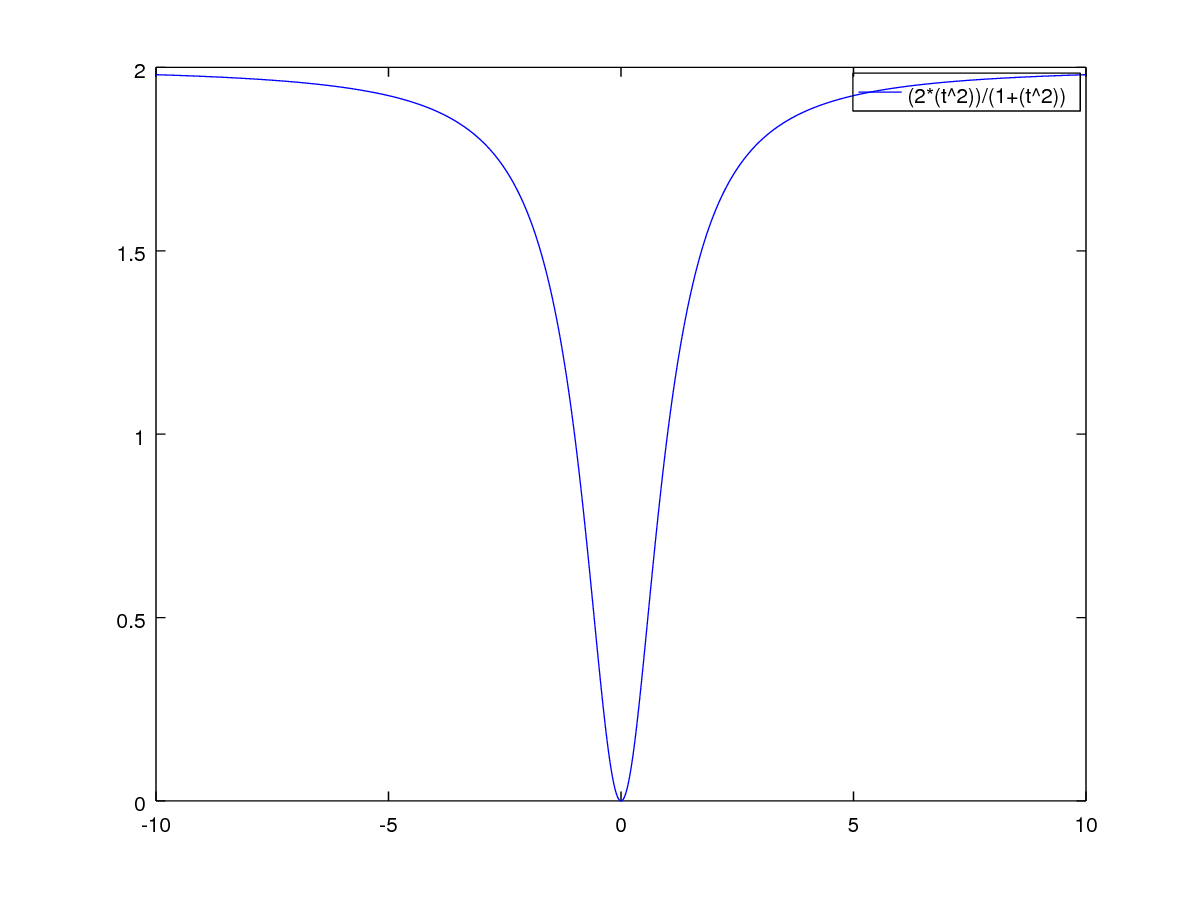
\includegraphics[scale=.5]{./lai.png}
  \end{figure}
\end{frame}

\begin{frame}
  \frametitle{Limits at Infinity IV}
Here is another important property of limits (call this \alert{Theorem
2}). If $1/x^{n}$ is defined and $n>0$, then
\begin{equation}
  \label{eq:faingiej}
  \lim_{x\rightarrow{}\infty}\frac{1}{x^{n}}=0\mbox{ and }\lim_{x\rightarrow{}-\infty}\frac{1}{x^{n}}=0
\end{equation}
\end{frame}

\begin{frame}
  \frametitle{Polynomial and Rational Functions}
A polynomial function looks like this,
\begin{equation}
  \label{eq:kaimeeyo}
  p(x)=a_{n}x^{n}+a_{n-1}x^{n-1}+\ldots{}+a_{2}x^{2}+a_{1}x+a_{0}
\end{equation}
For example, $p(x)=7x^{3}-4.7x^{2}+6$. $n>0$ is a natural number, and
the $a_{i}$ are called \alert{coefficients}. They are real numbers.
A rational function looks like this,
\begin{equation}
  \label{eq:raephoot}
  q(x)=\frac{p_{1}(x)}{p_{2}(x)}
\end{equation}
where $p_{1}(x)$ and $p_{2}(x)$ are polynomial functions. For example,
\begin{equation}
  \label{eq:yaingiaj}
  q(x)=\frac{5x^{2}-\pi{}x+9000}{e^{2}x+2}
\end{equation}
\end{frame}

\begin{frame}
  \frametitle{Limits at Infinity V}
When we are looking for the limit of rational functions as they go to
negative or positive infinity, we often get an indeterminate form.
\begin{equation}
  \label{eq:airoovae}
  \lim_{x\rightarrow\infty}\frac{x^{2}-x+3}{2x^{3}+1}=\frac{\infty}{\infty}
\end{equation}
Here is a technique that will almost always work. Divide both the
numerator and the denominator by $x^{m}$, where $m$ is the highest
exponent you can find.
\begin{equation}
  \label{eq:ahrahnei}
  \lim_{x\rightarrow\infty}\frac{x^{2}-x+3}{2x^{3}+1}=\lim_{x\rightarrow\infty}\frac{\frac{1}{x}-\frac{1}{x^{2}}+\frac{3}{x^{3}}}{2+\frac{1}{x^{3}}}=\frac{0}{2}=0
\end{equation}
\end{frame}

\begin{frame}
  \frametitle{Limits at Infinity VI}
Here are two more examples.
\begin{equation}
  \label{eq:ikiegeip}
  \lim_{x\rightarrow{}-\infty}\frac{3x^{2}+8x-4}{2x^{2}+4x-5}=\lim_{x\rightarrow{}-\infty}\frac{3-\frac{8}{x}-\frac{4}{x^{2}}}{2+\frac{4}{x}-\frac{5}{x^{2}}}=\frac{3}{2}=1.5
\end{equation}
\begin{equation}
  \label{eq:deegiech}
  \lim_{x\rightarrow{}\infty}\frac{2x^{3}-3x^{2}+1}{x^{2}+2x+4}=\lim_{x\rightarrow{}\infty}\frac{2-\frac{3}{x}+\frac{1}{x^{3}}}{\frac{1}{x}+\frac{2}{x^{2}}+\frac{4}{x^{3}}}=\frac{2}{0}=\mbox{undefined}
\end{equation}
In the second example, the limit does not exist. Sometimes, we write
$\lim_{x\rightarrow{}a}=\infty$ or $\lim_{x\rightarrow{}a}=-\infty$,
depending on which way the function goes.
\end{frame}

\begin{frame}
  \frametitle{Example I}
Consider the function,
\begin{equation}
  \label{eq:shuungae}
  f(x)=\frac{x-4}{\sqrt{x}-2}
\end{equation}
Let's find
\begin{equation}
  \label{eq:ailuiquo}
  \lim_{x\rightarrow{}4}f(x)
\end{equation}
\end{frame}

\begin{frame}
  \frametitle{Example II}
First, fill out the table:

\begin{tabular}{|l|l|l|l|}\hline
  $x=3$ & $f(x)= 3.7321$ & $x=5$ & $f(x)=4.2361$ \\ \hline
  $x=3.5$ & & $x=4.5$ &  \\ \hline
  $x=3.75$ & & $x=4.25$ & \\ \hline
  $x=3.9$ &  & $x=4.1$ & \\ \hline
  $x=3.95$ & & $x=4.05$ & \\ \hline
  $x=3.99$ & & $x=4.01$ & \\ \hline
\end{tabular}
\end{frame}

\begin{frame}
  \frametitle{Example III}
Next, let's assume that $x\neq{}4$ and expand both the numerator
and denominator by $\sqrt{x}+2$. Simplify
\begin{equation}
  \label{eq:oudiolee}
  g(x)=\frac{(x-4)\cdot(\sqrt{x}+2)}{(\sqrt{x}-2)\cdot(\sqrt{x}+2)}\mbox{ on domain }\mathbb{R}\setminus\{4\}
\end{equation}
Except on $x=4$, $g$ agrees with $f$. Determine
$\lim_{x\rightarrow{}4}g(x)$.
\end{frame}

\begin{frame}
  \frametitle{Exercises I}
Evaluate the following two limits.
\begin{equation}
  \label{eq:uheafaix}
  \lim_{x\rightarrow{}3}=\frac{\sqrt{x^{2}+7}+\sqrt{3x-5}}{x+2}
\end{equation}
\begin{equation}
  \label{eq:azeeghee}
  \lim_{x\rightarrow{}-1}\frac{x^{2}-x-2}{2x^{2}-x-3}
\end{equation}
\end{frame}

\begin{frame}
  \frametitle{Exercises II}
Evaluate the following three limits.
\begin{equation}
  \label{eq:haeceema}
  \lim_{x\rightarrow{}2}3
\end{equation}
\begin{equation}
  \label{eq:aogedish}
  \lim_{x\rightarrow\infty}\frac{3x+2}{x-5}
\end{equation}
\begin{equation}
  \label{eq:xaebiaph}
  \lim_{x\rightarrow\infty}\frac{x^{5}-x^{3}+x-1}{x^{6}+2x^{2}+1}
\end{equation}
\end{frame}

\begin{frame}
  \frametitle{Finding Limits Exercises}
Find the following limits,
\begin{equation}
  \label{eq:ixahngoo}
\lim_{x\rightarrow{}9}\frac{\sqrt{x}-3}{x-9}
\end{equation}
\begin{equation}
  \label{eq:etheshoh}
\lim_{x\rightarrow\infty}\frac{\sqrt{x^{2}-8x}}{2x+1}
\end{equation}
\begin{equation}
  \label{eq:chahgaew}
\lim_{x\rightarrow{}-1}\frac{x^{2}-x-2}{2x^{2}-x-3}
\end{equation}
\begin{equation}
  \label{eq:oofeegae}
\lim_{x\rightarrow\infty}\frac{2+\frac{1}{x+4}}{3-\frac{1}{x^{2}}}
\end{equation}
\begin{equation}
  \label{eq:yupeethi}
\lim_{x\rightarrow\infty}\frac{x-2x^{3}}{(1+x)^{3}}
\end{equation}
\begin{equation}
  \label{eq:reibaize}
\lim_{x\rightarrow\infty}\frac{\sqrt{4x^{2}+3}}{x+5}
\end{equation}
\end{frame}

\begin{frame}
  \frametitle{Limits Application}
In Einstein's theory of relativity, the length $L$ of an object moving
at a velocity $v$ is 
\begin{equation}
  \label{eq:aumiepha}
L=L_{0}\sqrt{1-\frac{v^{2}}{c^{2}}}
\end{equation}
where $c$ is the speed of light and $L_{0}$ is the length of the
object at rest. What is the one-sided limit of $L$ as $v$ gets
faster and faster?
\end{frame}

\begin{frame}
  \frametitle{Squeeze Theorem}
Sometimes you need some ingenuity to find a limit. Consider
\begin{equation}
  \label{eq:iepichae}
  \lim_{x\rightarrow{}0}\frac{\sin{}x}{x}
\end{equation}
% We can use the Squeeze Theorem and a geometric argument to find that
% this limit is 1 (see James Stewart, Single Variable Calculus, Sixth
% Edition, page 191).
\end{frame}

\begin{frame}
  \frametitle{Squeeze Theorem}
  If $f(x)\leq{}g(x)\leq{}h(x)$ when $x$ is near $a$ (except possibly
  at $x=a$) and
  \begin{equation}
    \label{eq:ohphaese}
    \lim_{x\rightarrow{}a}f(x)=\lim_{x\rightarrow{}a}h(x)=L
  \end{equation}
  then
  \begin{equation}
    \label{eq:quaighea}
    \lim_{x\rightarrow{}a}g(x)=L
  \end{equation}
\end{frame}

\begin{frame}
  \frametitle{Squeeze Theorem}
\begin{figure}[h]
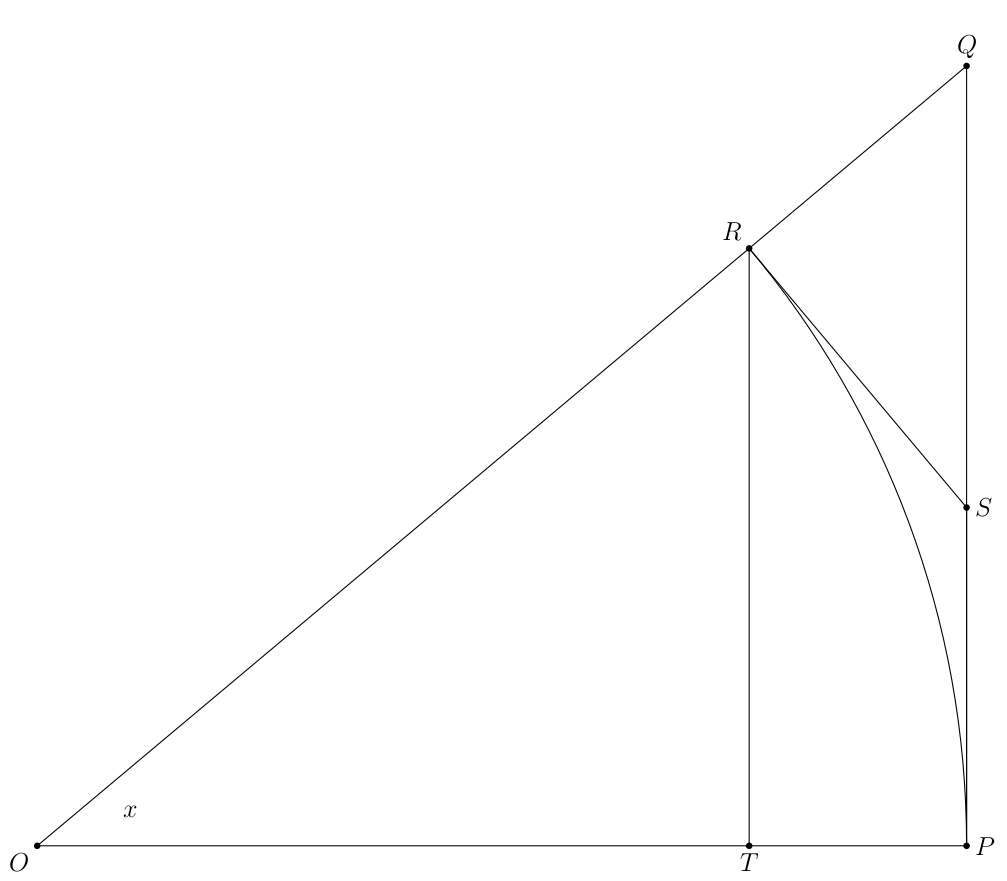
\includegraphics[scale=.24]{./limsinxoverx.png}
\end{figure}
\end{frame}

\begin{frame}
  \frametitle{Squeeze Theorem}
  In the previous slide, consider the unit circle with
  $\|\vec{OP}\|=\|\vec{OR}\|=1$ and the angle $x$ at $O$. For simplicity let's
  assume that $0<x<\pi/2$. The angle $x$ is also the length of the arc
  between $P$ and $R$. Consequently
  \begin{equation}
    \label{eq:iufoobue}
\|\vec{RT}\|=\sin{}x\leq{}x    
  \end{equation}
  and therefore
  \begin{equation}
    \label{eq:chaveeju}
    \frac{\sin{}x}{x}\leq{}1
  \end{equation}
\end{frame}

\begin{frame}
  \frametitle{Squeeze Theorem}
  Now consider
  \begin{equation}
    \label{eq:uraewiha}
    x\leq\|\vec{PS}\|+\|\vec{SR}\|\leq\|\vec{PS}\|+\|\vec{SQ}\|=\|\vec{PQ}\|=\tan{}x
  \end{equation}
$\|\vec{SR}\|\leq\|\vec{SQ}\|$ because the angle $QRS$ is a right angle.
(\ref{eq:uraewiha}) means that
\begin{equation}
  \label{eq:uebaenih}
  \cos{}x\leq\frac{\sin{}x}{x}
\end{equation}
Since $\lim_{x\rightarrow{}0}\cos{}x=1$ and $\lim_{x\rightarrow{}0}1=1$, we can use the squeeze
theorem, (\ref{eq:chaveeju}), and (\ref{eq:uebaenih}) for
\begin{equation}
  \label{eq:guabighe}
  \lim_{x\rightarrow{}0}\frac{\sin{}x}{x}=1
\end{equation}
\end{frame}

\begin{frame}
Here is a summary of methods to use to find limits.
\begin{enumerate}
\item If a function $f$ is continuous, then
  $\lim_{x\rightarrow{}a}f(x)=f(a)$.
\item If a function is composed of continuous functions, use the
  properties of limits (Theorem 1) to find the limit.
\item If the last step gives you an indeterminate form, try to factor
  either the numerator or the denominator and use the One Disagreement
  Rule. Example: $\lim_{x\rightarrow{}-2}[(x^{2}-x-6)/(x+2)]=-5$.
\item If there is a square root in a fraction, another thing to try is
  to multiply both numerator and denominator by the conjugate.
  Example: $\lim_{x\rightarrow{}-2}[(x-4)/(\sqrt{x}-2)]=4$.
\item For rational functions, use Theorem 2. Example:
  $\lim_{x\rightarrow\infty}(5x^{3}-x^{2}-x+3)/(2x^{3}+1)=5/2$.
\end{enumerate}
\end{frame}

\begin{frame}
  \frametitle{End of Lesson}
Next Lesson: Derivatives
\end{frame}

\end{document}
